\documentclass[a4paper,spanish] {article} 
\usepackage [spanish] {babel} 
\usepackage [latin1]{inputenc}
\usepackage{graphicx}
\usepackage{caratula}
\usepackage{subfig}
\usepackage{dsfont}
\usepackage{algorithm}
\usepackage{amsmath}
\usepackage{algorithmic}

\addtolength{\oddsidemargin}{-1in}
\addtolength{\textwidth}{2in}

\begin{document}
\pagestyle{headings}



\newpage

\materia{Aprendizaje por Refuerzos: Teor\'ia y Aplicaciones en Rob\'otica, Psicolog\'ia y Neurociencias}
\submateria{Tp Final}
\titulo{Desarrollo de algoritmos de aprendizaje y an\'alisis de resultados en una adaptaci\'on del problema Bomberman}

\integrante{Pablo Brusco}{527/08}{pablo.brusco@gmail.com}
\integrante{Carolina Hadad}{367/08}{carolinahadad@gmail.com}
\integrante{Sergio Medina}{333}{@gmail.com}
\integrante{Santiago Palladino}{138/05}{spalladino@gmail.com}
\integrante{Andres Taraciuk}{333}{@gmail.com}


\maketitle

		
\newpage
\tableofcontents
\newpage

\section{Objetivo}
	En  este Trabajo Practico nos interesa analizar el desempe\~ no de los algoritmos de aprendizaje aprendidos durante el curso,  aplic\'andolos  en un problema distinto de los vistos. En nuestro caso, elegimos adaptar el juego del Bomberman. 
	
	Compararemos los resultados del aprendizaje en agentes model-free y model-based, con los algoritmos de QLearning, RMax, RMax Factorizado, Sarsa y Sarsa Lambda, mostrando cu\'ales de ellos funcionan mejor en nuestro caso y a qu\'e se debe esto. Adem\'as analizaremos el efecto de aplicar rewards intermedios en el tiempo de aprendizaje del agente.
	
	Adem\'as veremos como varia el aprendizaje del agente al moverse en un ambiente estoc\'astico con mayor o menor grado de aleatoriedad.

\section{Introducci\'on}
	\subsection{Adaptaci\'on del juego del Bomberman}
	El juego que vamos usar es una versi\'on simplificada del juego del Bomberman. El objetivo del agente es llegar a la salida. El agente tiene 4 acciones de movimiento: arriba, abajo, hacia la izquierda y hacia la derecha. El tablero tiene paredes que obstaculizan su camino, algunas de ellas son rompibles y otras irrompibles. El agente tiene acciones para poner una bomba y para explotarla. Solo puede haber una bomba en el tablero, si el agente realiza una acci\'on de tirar bomba habiendo una bomba en el juego, la acci\'on no tendr\'a efecto. Al explotar la bomba se destruir\'an las paredes que est\'en arriba, abajo a la izquierda y a la derecha de ella. Si el agente estuviera en alguno de estos lugares o sobre la bomba, el agente muere, teniendo que empezar el juego nuevamente desde la posici\'on inicial. Nos interesa que el agente aprenda una pol\'itica para llegar a la salida realizando la menor cantidad de acciones posibles.	
	
	\subsection{Uso}
	Para correr el programa se debe correr el archivo

\section{Visualizaci\'on}
	
\section{Modelo Conceptal de la arquitectura}
	%pagina http://yuml.me/diagram/scruffy/class/draw
	%codigo [Manager| run()]->1[Task|start(); perform(action)]
	%		[Task] ->1[Environment|start(); performAction(action)]
	%		[Manager]->1[Agent | learn(); nextAction()]
	
	\begin{figure}[h!]
  \centering
    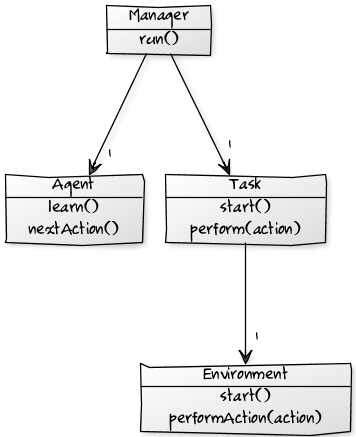
\includegraphics[width=0.5\textwidth]{MCarquitectra.png}
  \caption{Modelo Conceptual Arquitectura.}

	\end{figure}
\section{Algoritmos de Aprendizaje}
	Programamos agentes con pol\'iticas de aprendizaje distintas 
	\subsection{Agentes Model-Free}
		\subsubsection{QLearning}
		\subsubsection{Sarsa}
		\subsubsection{Sarsa ($\lambda$)}	
	\subsection{Agentes Model-Based}	
		\subsubsection{R-max}
		\subsubsection{R-max factorizado}

\section{Ambiente Estocastico}
	\subsection{Resultados}
	
 \section{Pol\'iticas de Refuerzo}
 	Para evaluar el efecto de aplicar pol\'iticas de refuerzos intermedios en el tiempo de aprendizaje de los agentes, incluimos los siguientes campos en el archivo de settings, que se agregan al refuerzo por llegar a la salida y al refuerzo negativo en el caso de que el agente muera. En el caso de que el agente llegue a la salida o muera recibe el WIN\_REWARD o el LOSE\_REWARD respectivamente, y no se agrega este refuerzo adicional.

\begin{description}
\item[NAVIGATION\_REWARD] Rewards por posici\'on del agente.
	\begin{itemize}
	\item NAVIGATION\_NO\_REWARD: No se agrega refuerzos intermedios adicionales.
	\item NAVIGATION\_REWARD\_PROPORTIONAL\_TO\_EXIT: Siempre que el agente realice una acci\'on que cambie su posici\'on recibe un refuerzo adicional proporcional a su distancia a la salida. En el caso de las acciones de movimiento que no cambien el estado, como por ejemplo intentar moverse hacia una posici\'on que tenga una pared, el agente no recibir\'a ningun refuerzo, de manera de desalentar este tipo de acciones. 
	
	Las formula para el c\'alculo de este refuerzo intermedio es la que sigue:
	$$ refuerzo = cercania\_en\_x + cercania\_en\_y $$
	donde
	$$ cercania\_en\_x =\mid MAP\_SIZE-1 -(EXIT_0 - agentPosition_0) \mid$$
	$$ cercania\_en\_y =\mid MAP\_SIZE-1 -(EXIT_1 - agentPosition_1) \mid$$
	siendo $EXIT = (EXIT_0, EXIT_1)$ la posici\'on de la salida en el tablero
	y $agentPosition= (agentPosition_0, agentPosition_1)$ la posici\'on del agente.
	
	Por ejemplo para un tablero de $8 \times 8$ con la salida en $(7,7)$ los refuerzos que recibir\'ia el agente al llegar a cada posici\'on ser\'ian estos:
	\begin{figure}[h!]
  \centering
    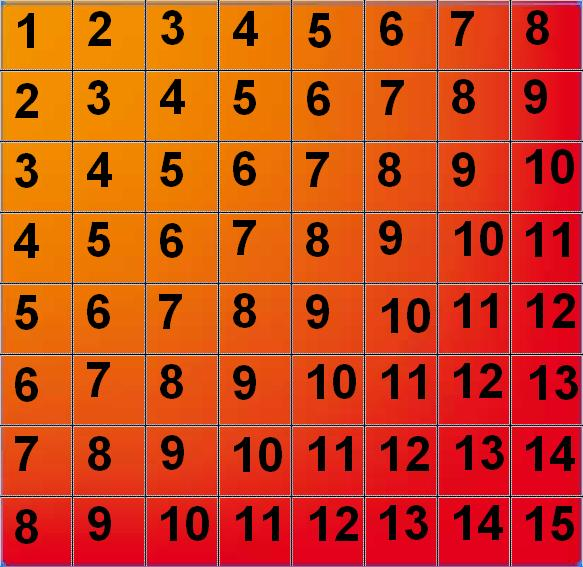
\includegraphics[width=0.5\textwidth]{refuerzos.jpg}
  \caption{Refuerzos para un tablero de 8 por 8 con salida en (7,7).}
	\end{figure}	
	La motivaci\'on de este refuerzo es que el agente trate de dirigirse hacia la salida.
	\end{itemize}

\item[BOMB\_REWARD\_POLICY] Rewards por destruir paredes.
	\begin{itemize}
	\item BOMB\_NO\_REWARD: No se agrega refuerzos intermedios adicionales.
	\item BOMB\_REWARD\_PER\_STONE\_DESTROYED: Cada vez que el agente destruye una pared, sin morir, recibe un refuerzo igual al BOMB\_REWARD del archivo de settings. La idea de este refuerzo es que el agente aprenda que debe destruir paredes.
	\item BOMB\_REWARD\_PER\_STONE\_DESTROYED\_PROPORTIONAL\_TO\_EXIT: el refuerzo anterior, usado solo podr\'ia hacer que el agente, por lo menos en las primeras iteraciones, intente romper muchas paredes. Por eso agregamos esta opci\'on, que le da mayor valor a romper paredes cercanas a la salida. La formula para este valor es $BOMB\_REWARD \times cercania\_a\_la\_salida$ calculando la cercan\'ia de la misma forma que antes.
	\end{itemize}

	
\item[NO\_ACTION\_NEGATIVE\_REWARD] Para desalentar el que el agente realizara acciones que no modificaran el estado, agregamos este booleano. Si se activa, cada vez que el agente realiza una acci\'on sin efecto, se le da un refuerzo negativo. 

\item[INITIAL\_REWARD] En la misma l\'inea que el \'item anterior, tambi\'en permitimos variar el refuerzo que se le da al agente al realizar cualquier acci\'on. La idea es que si este valor fuera negativo, el agente intentar\'a llegar lo mas r\'apido a la salida. Esta idea se integra al $\gamma$, pero permite explicitar el valor negativo de realizar acciones.

\end{description}

	Las funciones para la aplicaci\'on de estos refuerzos se pueden encontrar en el archivo $Rewards.py$ y son llamadas desde Task de acuerdo a las pol\'iticas elegidas por el usuario en el archivo de Settings.
 
\section{Pruebas y resultados}
	\subsection{Sin Rewards Intermedios}
	\subsection{Rewards Intermedios por posici\'on del bomberman}
	\subsection{Rewards Intermedios por explotar bomba}
	\subsection{Rewards Intermedios por explotar bomba relativo a la posicion de la bomba}

\section{Conclusiones}


	





		


		
		

		
		

	 
	
\end{document}